\documentclass[fonzsize=13pt,oneside,listof=totoc,paper=a4,headings=small]{scrbook}
% Nützliche Packages für die Gestaltung und allgemeine Konfiguration des Dokuments
\setlength\parindent{0pt}
% -----------------------------------

% Allgemeine Formatierungen
%\usepackage{ngerman}				% neue deutsche Rechtschreibung
\usepackage[utf8]{inputenc} 		% Umlaute im Text
\usepackage[T1]{fontenc}
\usepackage{xspace}                 % Vermeidung von "ineinanderfallenden f's", wie z.B. bei Schifffahrt
\usepackage{url}		            % korrekte Anzeige/Umbruch von URLs
\usepackage{listings}               % z.B. nützlich zum Einbinden von Quellcode
\usepackage{hyperref} 				% für Hyperlinks in PDF-Dokumenten 
\usepackage{lmodern}
\usepackage{enumerate}
\usepackage[onehalfspacing]{setspace}

% Kopfzeile
\usepackage[headsepline,manualmark]{scrlayer-scrpage}
\clearpairofpagestyles
\ohead{\pagemark}
\ihead{\headmark}
\automark{chapter}
\pagestyle{scrheadings}

% Seitenspiegel
\usepackage[left=25mm,right=20mm,top=25mm,bottom=25mm]{geometry}

% Literatur
%\usepackage[square,sort,comma,numbers]{natbib}         % Deutsches Literaturpackage
\usepackage{cite, float}
\usepackage{hyperref}

%\usepackage{float}
% Grafiken
\usepackage{graphicx} 				% Grafiken einfügen (pdf,png - aber jpg vermeiden)
\graphicspath{{./Bilder/}}          % Pfad zu den Bildern

% Tabellen
\usepackage{booktabs} 				% bessere Gestaltung von Tabellen
\usepackage{longtable} 				% für bessere Tabellen über mehrere Seiten

% Koma-Script Kompatibilität
\usepackage{scrhack}

% Das Dokument selbst mit seinen Bestandteilen
% --------------------------------------------
\begin{document}
\frontmatter 
% ----------------------------------------------
    % Titelseite soll keine Kopf oder Fußzeile haben
\thispagestyle{empty}



\vspace*{-20mm}
\begin{flushright}

\includegraphics[width=0.5\textwidth]{Bilder/LogoHS.png}
\end{flushright}


\vspace*{2cm}

% Alle Elemente sollen zentriert sein
\begin{center}
% Art der Arbeit => (Bachelorarbeit, Masterarbeit, Seminararbeit)
{\Large \textbf{Seminar Report}}\\ 

\vspace*{1cm}


{\large Game Engineering und Visual Computing (Master)\\[1mm]}

\vspace{1cm}

% Titel der Arbeit 
%{\Large \bfseries Graphische Effekte \\ 
%	zur Erzeugung einer \\
%	gewünschten Atmosphäre\\}

{\Large \bfseries Visual effects \\ 
    to convey a \\
    desired atmosphere\\}


\vspace{1.5cm}

% Name des/der Autors/Autoren
{\large Philipp Geirhos}\\[40mm]

\end{center}

\vfill

% Aufgabensteller, Kontaktdaten und Abgabetermin
\parbox{120mm}{
\begin{tabbing}
Aufgabensteller/Prüfer \hspace{.7cm} \= Prof. Dr. Christoph Bichlmeier\\
Arbeit vorgelegt am                  \> 09. Juli 2021\\
durchgeführt in der                  \> Fakultät Informatik\\[4mm]
% falls der praktische Teil der Arbeit in einer Firma durchgeführt wurde.
% Die Nennung des Betreuers ist freiwillig und mit diesem abzustimmen
\end{tabbing}
}

 				    % Titelblatt
    \newpage

\vspace*{1cm}

\begin{center}
    \textbf{Abstract}
\end{center}

\vspace*{1cm}

\noindent 
Atmosphere is one of the most memorable aspects of video games. It describes the feeling of a particular game and how it is remembered by the user. Although it is strongly linked to the commercial success of a video game, game atmosphere has not received much attention in scientific research. It is in fact not even clearly defined in the literature. Therefore, this term paper will first try to provide a clear definition of the term "game atmosphere". Then, some techniques are discussed to create a desired atmosphere by changing and composing the visual effects and especially the lighting in a scene. Finally, some techniques to create a desired atmosphere will be illustrated on a serious game that was developed in parallel to this thesis.   	% Abstract
    \tableofcontents 					            % Inhaltsverzeichnis
    \clearpage
\mainmatter 						% die einzelnen Kapitel, bei Bedarf weitere *.tex Dateien erzeugen und hier einbinden
    \chapter{Introduction}
As stated by Ribeiro et al, the term game atmosphere is used to describe "a subtle but important, intangible, generally aesthetic quality in games that leads to emotional immersion."\cite{Ribeiro.2020}. He derived this definition from several game reviews that were described as atmospheric, with these reviews referring to games such as Metro: Last Light, Limbo, and Firewatch. 
Furthermore, in a presentation at the Games Developer Conference (GDC), game designer Greg Kasavin, who worked on games such as Bastion tried to break down the concept of game atmosphere into a few technical aspects: He notes that atmosphere consists of thematic cohesion, internal consistency, and specific details \cite{GDD}.\\

However, in the same paper, from which this definition originates, it was also said in the same course that the concept of atmosphere in games is not the subject of many academic papers or research efforts. And although companies are slowly publishing scientific papers on the subject, it is mostly left to the artistic vision of a game studio or a designer.\cite{Ribeiro.2020}.
\\
Although a clear definition and also many scientific works on the subject of game atmosphere are missing, factors can be derived which clearly contribute to the atmosphere: visual design, story and how it is written, as well as the sound and music design \cite{MDA}.
\\
Therefore, this seminar paper deals with exactly this topic and tackles the first aspect of game atmosphere: The question of how visual effects and the use of lighting can be applied to achieve a desired atmosphere in games. First, many fundamental mechanics are explained, which are necessary to understand how lighting works in real life. This basic knowledge is necessary to venture into the virtual world and see how these fundamental properties are applied there and thematically adapted for a desired atmosphere. Once an appropriate set of tools has been established, it will be considered how these principles can be applied to a serious game developed in the context of this seminar work.

\section{Motivation}
Game atmosphere is one of the most important aspects a game has to offer \cite{Ribeiro.2020}. In his article for the website "Gamasutra", the game developer Matthew Bentley summarized the feeling of a dense atmosphere very well and fittingly: "Atmosphere is the feeling that remains when the rest of the game shuts the hell up" \cite{Gamasutra}. So the goal is to use visual effects to create a feeling for the player that is long lasting and can be conveyed to them without the use of other gameplay elements. \\

To accomplish this, however, a basic understanding of lighting itself and how it works in the real world must first be established. Only then is it possible to understand techniques used by lighting designers in all kinds of media. In addition, it is then possible to make use of the varied literature that exists for real lighting, as this can be applied to a very large extent to the design of video games\cite{Niedenthal1404353}. 
    \chapter{Simulated Illumination and Tension in Games}
As established earlier, the lighting of a given scene can greatly define the atmosphere in a game. However, to discuss some lighting techniques and rules, one first has to define the vocabulary that is used to describe the behavior of light in a video game.

\section{Translating from reality to games}

Simulated illumination is defined as the method by which virtual (3D) game environments are rendered taking into account all lighting information in the scene.\cite{Maggi.2006} Of cause, the style of these simulations are not set in stone and can range, depending on the capability's of the game engine and the artist's vision, from very stylized to nearly photo-realistic. In an effort to define such vocabulary for the lighting of a scene, light designer Louis Clair first laid out some characteristics of lighting in the real space.\cite{Niedenthal1404353}:

\begin{enumerate}
    \item \textbf{Brightness or luminance} \\
    In the real world, this can be measured in lux or lumens. This depends, whether the light is measured at the receiving surface(lux) or at the source (lumen) \cite{LuxAndLumens}
    \item\textbf{Color} \\
    Can be expressed through the color rendering index \cite{colorrendering}, measured through degrees Kelvin, specified through chromatic diagrams or even verbal descriptions
    \item \textbf{Direction, distribution, and movement from the source} \\
    This can be indicated with a system of arrows or with a lighting distribution diagram \cite{dmlights}
    \item \textbf{Shadow quality}\\
    The density and quality of hard or soft shadows and their edges.
    \item \textbf{Contrasts}\\
    The Contrast between different layers in a given room.
\end{enumerate}



While not all these measures are relevant or even possible to implement in digital lighting simulations \cite{Niedenthal1404353}, all of them can be taken into account by a lighting artist for virtual environments in modern engines. 

Using the above characteristics, the color of a given light, for example, can be specified by an RGB-Value. The direction and distribution can be set by using different forms or combinations of light emitters such as point lights, spotlights and directional (parallel) lights. Spatial contribution, speed or luminance can be accessed through the games code and contrasts can be, if not generated to the artist's liking, be manipulated by post-processing effects. 
\newpage
For designing such a light simulation (or any other simulation for that matter), one has to make choices, which define the arrangement, setting and configuration of lights in a virtual Scene. Therefore, Simon Niedenthal describes four key steps of the process of developing such a simulation\cite{Niedenthal1404353}: 

\begin{enumerate}
    \item Acquisition of source information about the subject
    \item Selection of key characteristics and behaviors of the subject
    \item The use of simplification, approximations and assumption within the simulation
    \item Fidelity and validity of the simulation outcome has to be confirmed
\end{enumerate}

By executing, and therefore implementing, these steps, it becomes obvious, how lighting algorithms have evolved over time. The Step of acquiring information about a given scene dates back even to the 9th century. Ranging from Arab philosopher Al. Hazan (specular reflections) over Newton, who formulated the inverse square law used to calculate the falloff of light intensity to Lambert (1760) (diffuse reflections). \cite{Niedenthal1404353}. 

Complex characteristics (2) of lighting are developed in relatively recent years. An early example of such, more complex, technique is  color bleed, which first has been rendered by Goral et al. in 1984 \cite{Goral84} 

The complexity of light simulations, even when kept relatively simple, has introduced a tight performance budget and therefore many simplifying algorithms (3) had to be used to ensure a reasonable framerate for real-time simulations. Early lighting algorithms focused on the recreation of direct light effects and didn't take more complex shading and indirect lights into account \cite{Niedenthal1404353}, Historically, this tight budget of processing introduced by the complexity of a lighting simulation has drastically limited the number of light sources and fidelity of effects that could be used in a scene for a real-time simulation of light (aka. video a game). Only in recent years, the capability of real-time engines and computer hardware had created enough headroom to loosen the performance budget a bit and create more variant graphical effects and lighting techniques \cite{Niedenthal1404353}. An example of this is the rise of real-time ray tracing, which was first implemented by Nvidia and then also by AMD for real-time graphics. This allows for the simulation of indirect light and global ambient occlusion with a relatively low tax on the performance budget \cite{RTXON}. This, in turn, has significantly increased artistic freedom and enabled more versatile and elaborate levels. 

The validation step (4) is, in many cases, the hardest to execute, since video games are, more often than not, creating a space, which does not exist in real life. However, Goral, for example, validated his algorithm for color bleeding by comparing his computer-generated render and its RGB values at certain places with a real-life representation of the same scene. The real-life color values were taken with photometric readings. \cite{Goral84}. In the case of computer games, this step of validation is also often a play test, in which it is asked whether the player experiences the desired emotion and whether the desired atmosphere is created. 
\newpage
\section{Using simulated illumination as a design material}

Light and therefore design of lighting effects has long been seen as the basis of our perception of space and form. This is true for many media besides video games such as film, theater or computer animation. In recent years, especially with the ever-lasting rise of processing power and capability of lighting algorithms light has been used to convey a deeper design aspect: Light can be used to manipulate, how a player sees a scene and how he reacts to it. It can manipulate feelings and has a deep connection to the player's emotions. Moreover, it can be used to create a more believable and dramatic environment for the player to immerse himself in. Therefore creating a much deeper and defined atmosphere. \cite{Shadowplay}
\\\\
The creation of such immersive and visually rich lighting setups for game environments leaves the game developer with a great deal of artistic freedom. Unlike in other lighting design tasks (as for example in architecture or theater), game lighting has to be created entirely from scratch. Every surface, form and character has to be considered and has to blend in the rest of the scene. Given these differences, a light designer might be tempted to only focus on the end result (the rendered frame) and disregard the spatial relations and placements of each light source. However, due to the dynamic nature of video games, the player can alter his position in a scene, which leads to a completely different lighting situation, which the lighting designer also has to take care of. \cite{Niedenthal1404353}
\\\\
Currently, lighting practices for the creation of 3D environments in video games, are heavily inspired by traditional media such as animation, film, theater and even architecture. This is, in part, due to the lack of specific research on game lighting and interactive scenes \cite{Maggi.2006} and the similarities, which are existent between the design of a traditional, static, scene and an interactive scene in a video game: A light designer of an interactive scene still has to stage lights in a three-dimensional environment, identify attributes such as color, intensity, spacial contribution and shadows and thereby setting the desired atmosphere of a virtual scene.
\newline
To define the goals of a lighting setup in virtual scenes, Sharon Callahan, a lighting designer at Pixar proposed five design goals for creating a synthetic scene\cite{Storytelling}: 
\begin{enumerate}
    \item Directing the viewer's eye
    \item Creating depth
    \item Conveying time of day and season
    \item Enhancing mood, atmosphere and drama
    \item Revealing character personality and situation
\end{enumerate}
\newpage
So as seen, the process of designing a lighting setup for interactive media contains two elements: At first it is descriptive for the user. It helps him to "make sense of the scene". It accomplishes that by highlighting important items, guiding his way to the next passage to progress in a story or a task or simply adding readability to his surroundings. 
The other element, and focus of this seminar report, is to convey a deeper meaning. Lighting can be (and is) directed towards the players emotion and understanding of narrative structures. These five design goals all support components of a players experience in a video game: attentiveness, absorption,
coherence, emotion and "make-believe",\cite{Niedenthal1404353} thus creating a game's atmosphere. 
Those design goals largely reflect Pixar's influence on lighting research in virtual scenes. In a video game, however, the player can take as much time as he wants to experience, manipulate and investigate the lights in a scene and the work that went into it\cite{Maggi.2006}. Thus it opens up the opportunity to explore the emotional content of designing lights in interactive media. 

\section{Designing the lighting simulation}
\subsection{Drawing upon experience from other media}
In his book "The Language of New Media" from the year 2000, Lev Manovich states, that "the visual culture of the computer era is cinematographic in appearance". This, for the most part, still holds true. As established above, game creators use a filmic vocabulary when creating a lighting arrangement in virtual scenes. Game elements such as cut scenes clearly suggest the use of these, already established, therms. Moreover, certain larger lighting strategies such as face lighting conventions, time of day, narrative elements and mood translate really well to the filmic approach \cite{Shadowplay}. Obviously, however, many elements of game lighting can not be transferred to the filmic approach. Traditional media, animated or in life-action, are from a fixed perspective and the light is directed to this one perspective. Games however are an interactive medium and allow the player to explore the scene from many different angles and different timeframes \cite{Maggi.2006}. Thereby, it makes sense to compare the process of designing lighting in a game to the work of an architectural lighting designer. Grodal even points out, that video games evoke first-person emotions rather than third-person emotions. Accordingly to him, this happens because games implement some motion controls to interact with the player and thus simulate real-world patterns of interactions \cite{Grodal}. 
\newpage
\subsection{Drawing upon experience of real spaces}
Brenda Laurel said in her work "Computers as Theater", that we always take a subset of our senses with us, when we engage in virtual environments. Following this argumentation, it can be claimed, that virtual experiences, at least in part, can be translated to our real-world experience, when exposed to a carefully set up light scene. Of cause the player's experience, when confronted with a virtual scene can not directly be translated into a real-world experience. Virtual experiences are  (in most cases) transmitted through a flat-screen occupying only a portion of our field of view and having limited space of colors whits intern limits the range of the simulated illumination. \cite{Niedenthal1404353}. Nevertheless, according to Gibsen, our encounter with light, even in a virtual environment, still triggers a direct response to its light; “a picture,” he writes, “is a surface so treated that (it) contains the same kind of information that is found in the ambient optic arrays of an ordinary environment” \cite{Gibson71}.
If we accept this and see simulated illumination as related to real illumination and its triggered reaction, we can benefit off of many types of research, that have been conducted for real-life lighting and its effects on the human. Many (though obviously not all) can be reused for information on how to light virtual scenes. Much research in the past tries to establish a standard of how much and which light best supports intense visual tasks in work and public spaces \cite{Niedenthal1404353}. An additional example is Kenz, who researched during his study conducted in 2001 the effects of not directly visible illumination upon the emotion of a subject \cite{Knez2001}. Knez even has proposed a link between the temperature of lighting (red and blue) and the mood of a player and discovered different emotional reactions to these temperatures of color. These finding's indeed not only introduce a new approach to the study of visual effects and their simulation. It also opens up new potential for designing the lighting in a game to trigger certain physical responses which help the player to immerse himself in the scene. 
\newpage
\subsection{Designing lighting in a video game}
\label{chap:witcher}
When looking at video games and their lighting it becomes obvious, that we can not only rely on experience made in the real world and research from other forms of media. To elaborate this, "The Witcher 3" from the polish company CD Project RED is taken as an example. This game gives the player the mechanic to toggle an ability to view extra hints, clues and objects in the game world. This is conveyed by an overlay (see Figure \ref{fig:witcher}), which is not orientated by any traditional forms of light design or visual effects. \cite{witchersenses}

\begin{figure}[h]
	\centering
		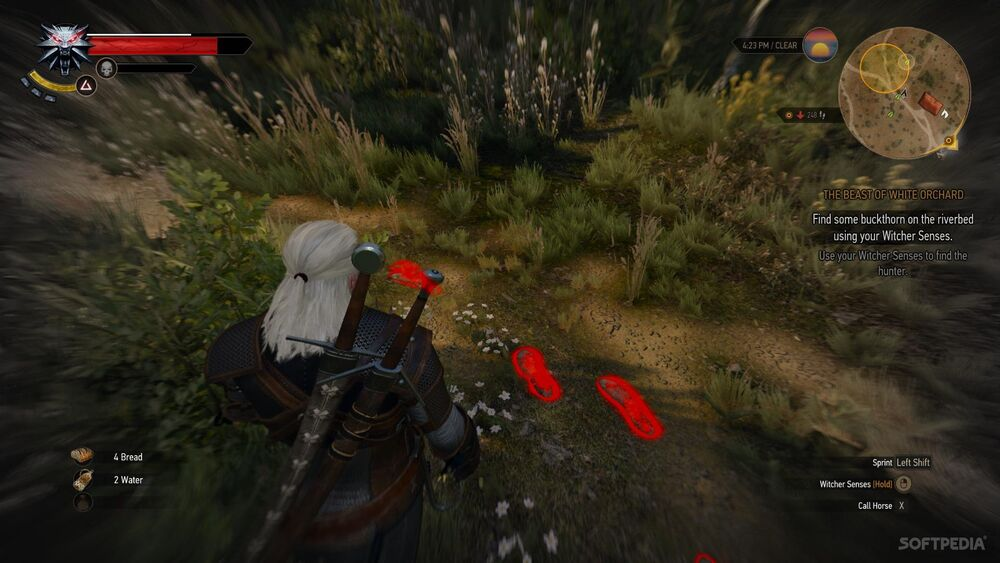
\includegraphics[width=0.9\textwidth]{Bilder/The-Witcher-3-Diary-Witcher-Contracts-Are-Quite-Fun-482236-2.jpg}
	\caption{The "Witcher Sense" in the game The Witcher 3 \cite{witchersenses}}
	\label{fig:witcher}
\end{figure}

It gives the player the possibility to visualize objects in the game scene, that are are not visible using common means of visible light. These include highlights of objects and tracks, that are important clues to solve a puzzle, the player is confronted with. These visual effects can also mark enemies or other dangerous entities. This lets the player, with the press of a button, completely change the visual appearance of the game. In this case, it is even an unnatural, not found in any real observations or literature, style. Another example of a specific challenge of light design, which is only applicable to games and other forms of interactive media is the active manipulation of light by the player. For example, Flashlights can drastically alter the mood and the player experience of the player within a virtual scene and the way the player interacts with a given scene \cite{Shadowplay}.
\newpage
In summary, the interactive nature of a video game both widens the designer's possibilities to create rich and compelling atmospheres but also imposes new concerns and design guidelines that have to be taken care of. Simon Niedenthal, therefore, laid out 3 considerations for a lighting designer working on interactive virtual scenes to be made \cite{Shadowplay}: 

\begin{enumerate}
    \item \textbf{Defining the basic characteristics of the illumination of the environment in time and space}\\
    Even if the player might has the ability to alter the lighting of a virtual scene by adding light (e.g. with a flashlight or car headlights) or subtracting light (e.g. by shooting out lights or blocking sources of light), the designer has to create a base lighting for his scene. This can consist of a base ambient lighting, essential shadows and their density and quality, or outlining the visual features of the world. Here he can apply some techniques used in film and other static types of media such as "high-key" or "low-key" (elaboreted in section \ref{cap:highLow}) strategies. High-key traditionally is associated with comedy and lighter fare whereas low key is most commonly associated with horror, survival and more dramatic scenes. 
    
    \item \textbf{Outlining the capabilities of the player}\\
    As described above, in the game "The Witcher 3" the game scene can be drastically altered by the abilities of the player and therefore presented in a whole different visual style. Offering the player a set of choices, which are communicated through the use of visual effects and lighting. In this case, it conveys a sense of mastery over the environment and other characters within the game. Other examples however can also convey a sense of vulnerability: In the Game "Splinter Cell" the player's flashlight can uncover important entities within the game world, but can also alert enemies.
    
    \item \textbf{Integrating illumination concerns within the game's experience}\\
    The lighting artist has to integrate the lighting in the feel of the game. The visual effects have to harmonize with other aspects of the game's design (for example sound). This step also includes making player actions meaningful and to create a coherent experience for the game as a whole and therefore creating a believable and dense atmosphere. 
    
\end{enumerate}
\newpage
\section{The influence of virtual lighting on game worlds} \label{cap:simu}

To describe a simulation of light as good as possible, one can say, that it "visually describes game environments and brings them out of formlessness" \cite{Niedenthal1404353}. However, as already established in early sections of this work, digital lighting in video games opens up much more potential and enables the game's designer to convey higher-level emotions and atmospheres to the player. In his work "Complicated shadows: The aesthetic significance of simulated illumination in digital games" Simon Niedenthal proposes six design influences that have a direct impact on the player's experience of a game and thus its atmosphere. These will be elaborated within the following chapter and ordered. Each will have a greater impact on the player's sense of atmosphere than the last. 

\begin{enumerate}
    \item \textbf{Exposure} (direct experience of light qualities in virtual environments) \\
    As established in early chapters, specific illumination patterns have the ability to influence our subconscious feelings. "When we are exposed over a period of time to light, qualities such as brightness or color have the ability to affect our emotions and behavior. This occurs through activation (how aroused we become), as well as affect, or mood (Knez 2001)\cite{Knez2001}" That means, when specific lighting combinations predominate in virtual, interactive, environments, we can expect certain contributions to the players affection mood and atmosphere \cite{Shadowplay}.

    \item \textbf{Contrast} (variations of light qualities within the visual field)\\ 
    It is unlikely that the player will be confronted with a scene that has only one source of illumination or is homogeneously lit. Most of the scenes the player will be confronted with are built from a variety of elements, such as different light colors, natural and artificial light, shadows and etc. Our perception of contrasts, which are expressed through light differences in the scene, is one of the main mechanisms by which scenes are perceived and understood. For example, as mentioned earlier in Callahan's design goals, contrast is one of the main ways in which the player's attention can be drawn.  \cite{Storytelling}
    
    \item \textbf{Temporal change} (as a function of player navigation from environment to environment, as well as external influences) \\
    Many light effects and elements are perceived by the player only through a temporal shift. The design language is only revealed when the player moves through a level or waits for some time. Examples include the difference between day and night, light and dark, and warm and cold. Longer-term lighting changes can also be used as a stylistic device in games, for example, to convey progress or the story. By holding back or highlighting some lighting changes, the player's emotional experience is also pushed further. Generating a denser atmosphere. \cite{Niedenthal1404353}
    
    \item \textbf{Lighting patterns and conventions} (recognition of illumination patterns from other games and media types, genres, characters, etc) \\
    A closer look at the transfer of a lighting atmosphere from the real world to the virtual one quickly reveals a number of procedures from other media and games. These occurrences describe an impression that we associate with the atmosphere of a certain genre or the emotions of a certain image. As Callahan noted, these lighting and visual effects have the potential to illustrate the character and personality of a figure or even a scene. Thus they contain important tools and techniques to properly design the visuals of a game \cite{Storytelling}
    
    \item \textbf{Lighting effects} (moments at which the player becomes aware of light qualities, either to enhance the immediate game environment or to engage Atmosphere)\\
    In video games, there are often individual moments in which visual effects become particularly obvious. These effects are often used, for example, to draw attention to certain parts of the environment. This is the case, for example, with the so-called "godrays", which showcase the impact of light in a weaker lit part of the scene. Light effects can also be assigned a metaphorical function, for example in the game "Shadow of the Colossus", in which a light shine emanates from talking characters. \cite{Niedenthal1404353}
    
    \item \textbf{Interaction and player agency} (strategic or tactical player activity related to lighting, or lighting that serves as a feedback device for player action)\\
    Quite often, a player is not simply confronted with predetermined lighting, but can actively help shape it. For example, as seen in the example of the "Witcher senses" in "The Wither 3" (see Figure \ref{fig:witcher}), a supernatural ability can be illustrated, which gives the player a feeling of superiority. Lighting can also be used tactically, as in the case of Splinter Cell: In this stealth game, lights are shot out to further envelop the player in protective darkness. 
    
\end{enumerate}

The methods described above give the artist a variety of tools to enhance and develop the aesthetics and the atmosphere as well as the involvement of the player.
    \chapter{Using visual effects}

As already described in the last chapter, the games industry is often inspired by the film industry's research on lighting. Even, if in the last years, the game industry more and more started to conduct its own research on lighting and its effect on the players emotions and the games atmosphere \cite{Niedenthal1404353}. The film industry however already has its own research, that is well established in field. For this reason, this chapter will focus on the work an a Pixar lighting designer. The examples will therefore be taken from her work on "A Bugs Live" and "Toy Story 2" which she documented in her paper "Visual Storytelling through Lighting" \cite{sudeep}.

\section{Spacial lighting of virtual scenes}
\label{chapter:ThreePoint}
During the initial, static lighting of a virtual scene, it is important that the characters and elements that are placed in it blend in well with the environment. This not only makes the scene appear more believable but can also contribute to the creation of the desired emotion towards a character or even the entire scene.  The following is an excample of the use of the "Tree-Point-Lighting"-technique: The character is illuminated by 3 separate light sources (see Figure \ref{fig:woody} that are inserted into the environment. These are the key light, i.e. the light that primarily illuminates the character and has the largest share in the design (about two-thirds). This light usually emanates from the direction of the camera and is used to make prominent characters or subjects stand out in the scene. Also, the clever positioning of this light source can suggest or even define the personality of a character well. \\
The fill light is a weak but global light that illuminates the entire subject and gives some visibility to areas that would otherwise be completely shadowed. Fill lights are diffuse, which means that they do not cast a shadow or otherwise give the object a different structure. In the field of video games, this type of lighting is often called ambient light. \\
Finally, the backlight is used to make the subject stand out from its background. The most commonly used backlight, particularly in films, is the so-called rimlight. It is placed behind the character and provides a border around the subject, which significantly increases the readability of the scene for the viewer. However, since video games are an interactive medium, this light is often not generated by a direct light source, but by using shaders that approximate the result. 
\begin{figure}[H]
	\centering
		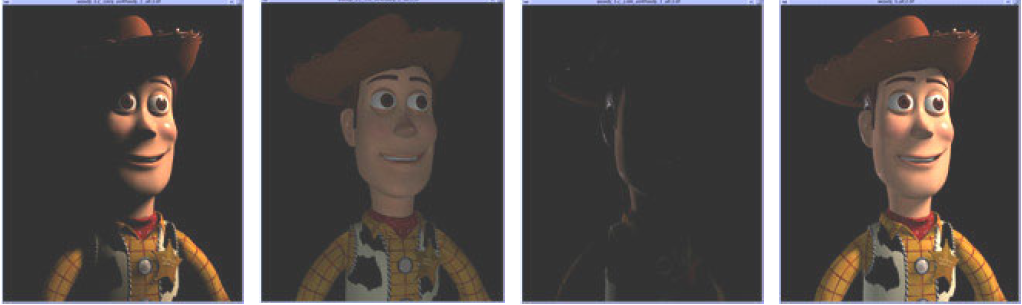
\includegraphics[width=0.7\textwidth]{Bilder/pixar keyrimfill.PNG}
	\caption{The use of Key, Fill and Rim Lights on Toy Story 2 \cite{sudeep}}
	\label{fig:woody}
\end{figure}

Often, in addition to the lights already mentioned, other sources of illumination are used to integrate the scene and its subjects. One of these is the "kicker light". It is usually placed on the opposite side of the key light and illuminates the corners of the subject that are not already covered by the key light. The main benefit of this type of lighting is to make the character or subject appear more three-dimensional. \\\\
Another light source often used is the "bounce light". These lights simulate reflections on subjects coming from other objects or another light source. Often these reflections are created by the real-time engine anyway, but the character and atmosphere of a scene can be adjusted separately. This can also suggest a more diverse scene to the player as is actually the case. \\
The following example (See Figure \ref{fig:teapot}) shows an example of how a virtual scene could be illuminated. It should be noted that this example is based on a static scene. Nevertheless, this lighting model is also possible for dynamic scenes, but the subject should then not be in the direct vicinity of the player, otherwise, there will be large changes in lighting \cite{Niedenthal1404353}. 
\begin{figure}[H]
	\centering
		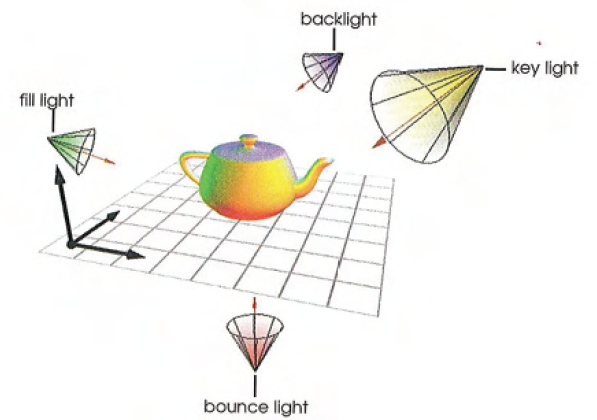
\includegraphics[width=0.7\textwidth]{Bilder/teapot.PNG}
	\caption{How a virtual scene may be lit \cite{Niedenthal1404353}}
	\label{fig:teapot}
\end{figure}
\newpage
In addition to the pure positioning of the lights, a number of other parameters of a light source can of course be set. The most obvious of these parameters are those that we already know from the real world, such as the color of the light, the brightness or the specularity. \\
The direction in which the light radiates can also be adjusted and parameterized by selecting the artificial light bodies. Possible are parallel, point, area and spotlights \cite{Shadowplay}. By carefully combining these, you can bring a scene to life and convey its atmosphere.\\
Even the form of light can, in case of area or spot light, be manipulated (see Figure \ref{fig:cookie}. This is done by using cookie textures, which act like a mask for the light source. This means that even complex patterns can be realized relatively easily in a virtual scene.
\begin{figure}[H]
	\centering
		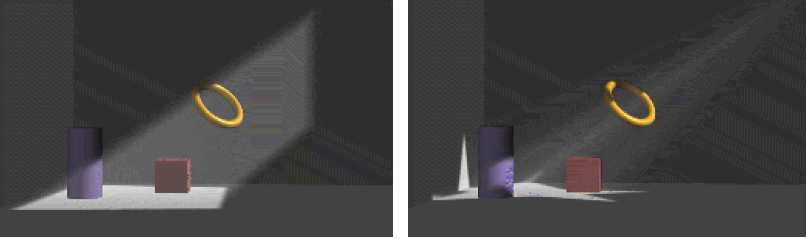
\includegraphics[width=0.7\textwidth]{Bilder/cookie.PNG}
	\caption{Using a cookie texture to modulate the appearance of a spotlight \cite{sudeep}}
	\label{fig:cookie}
\end{figure}

An additional immense advantage we have in virtual scenes is that virtual lights physically do not exist. This means that, unlike real films and their scene construction, we can place light sources anywhere in the scene. Another example for this is, that virtual lights can be programmed to have no fallof or to generate no shadows \cite{framework}\cite{sudeep}.

\section{Visual Styles}
\label{cap:highLow}
From the above methods, a quasi-infinite combination of illuminations can now be derived. For this reason, some categories were created to represent different styles \cite{Niedenthal1404353}. Lighting styles are described in terms of their tonal range, that is, the range of values from the darkest to the brightest light and the gray values in between. Lighting styles are also described in terms of the overall color, motivation, placement, and quality of highlights and shadows. \\

The character and mood of an image are significantly influenced by the tonal range from light to dark and by its distribution within the image. Those design decisions are decided early in the design process of a game or film. These decisions are usually motivated by the desired dramaturgy of the story and can be consistent throughout the time span of a scene or vary depending on the location and time of day or actions the player made on a given scene \cite{Niedenthal1404353}. While most of the categories and terms used to describe the lighting of a scene come from film and photography, many can be directly applied to the design of virtual scenes in video games. Two of these categories, which have a strong impact on the atmosphere of a scene, are high and low key lighting. These will be explained in more detail in the following paragraphs. 

\subsection{High-Key Stlye}
A light-hearted or comedic story might require a high-key lighting style. High-key lighting is a light setup for a scene that is predominantly well-lit with lots of soft fill light and mostly no harsh or shadows. The backgrounds, characters and set pieces also tend to be bright in color. That doesn't mean there are no dark areas, but the overall brightness tends to be light, the contrast is low, and the dark areas are soft and discreet. The result minimizes tension, as little is left to the imagination of the viewer or player\cite{Niedenthal1404353}. Which, in most cases, generates a light and relaxed atmosphere \cite{Storytelling}.

\subsection{Low-Key Style}
At the other end of the spectrum is low-key lighting. In a low-key lighting setting, most of the scene is darkly lit, with emphasis on the few areas that are brightly lit. The backdrops and costumes are usually darkly colored as well. The scene has a dark but not murky appearance. What is seen is as important as that which is not seen. The detail that is only hinted at is much richer than it would be with good lighting, this leaving a great deal of imagination left for the viewer or player and thus creating a more suspicious atmosphere \cite{Niedenthal1404353}. Light is used to direct the viewer's attention, darkness to stimulate his imagination \cite{Storytelling}.

\begin{figure}[H]
	\centering
		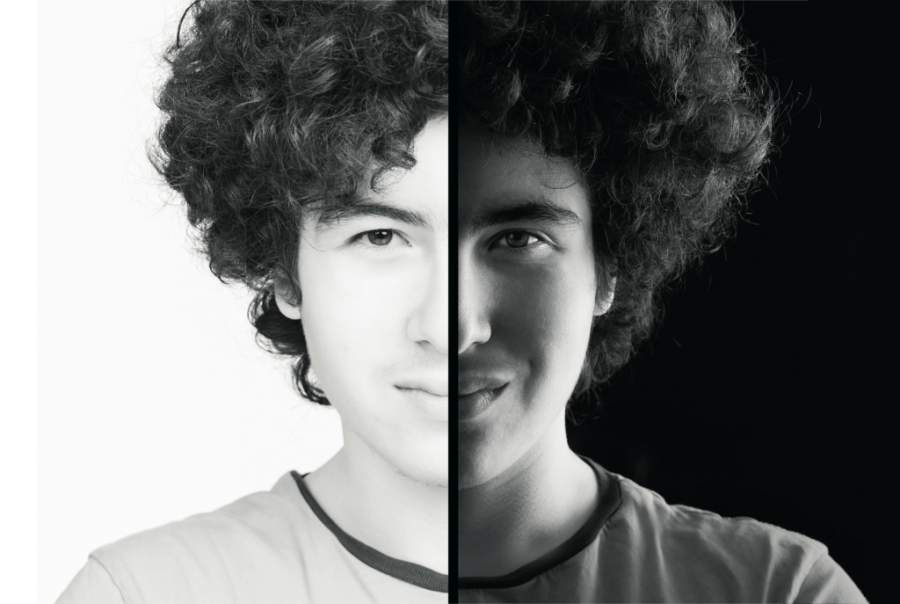
\includegraphics[width=0.7\textwidth]{Bilder/LowHighKey.jpg}
	\caption{High-Key (left) and Low-Key (right) lighting \cite{heisse}}
	\label{fig:cookie}
\end{figure}

Even before the viewer has understood the storyline, the lighting style can convey a feeling of a scene, especially when compared to scenes adjacent to it.Or within a single shot, one character can be modeled in light tones and another modeled in shadows and dark tones to suggest their individual personalities or their emotional or dramatic situations. This gives the viewer a first impression of the scene, which greatly affects the atmosphere and his feeling towards it\cite{Storytelling}.

\section{Creating Atmosphere through visual storytelling}
We can now examine how lighting develops and reinforces a story. As mentioned in the last chapter, the role of lighting can be roughly divided into the following  points \cite{sudeep} \cite{Storytelling}:

\begin{itemize}
    \item Directing the viewer’s attention
    \item Establishing a mood and atmosphere
    \item Creating a sense of depth
    \item Maintaining visual continuity
\end{itemize}

The main goal of lighting is to \textbf{guide the viewer's attention}. Lighting can be used to organize and prioritize elements and areas as well as characters in a scene. As Sudeep Rangaswamy has pointed out, effective lighting can divide a confusing scene with many distractions into individual, easy-to-understand areas \cite{sudeep}. Often the already established "three-point lighting" technique is used: A character is set off from his surroundings and background, which draws the viewer's attention strongly to him (see Figure \ref{fig:hopper}) \cite{Storytelling}. 

\begin{figure}[H]
	\centering
		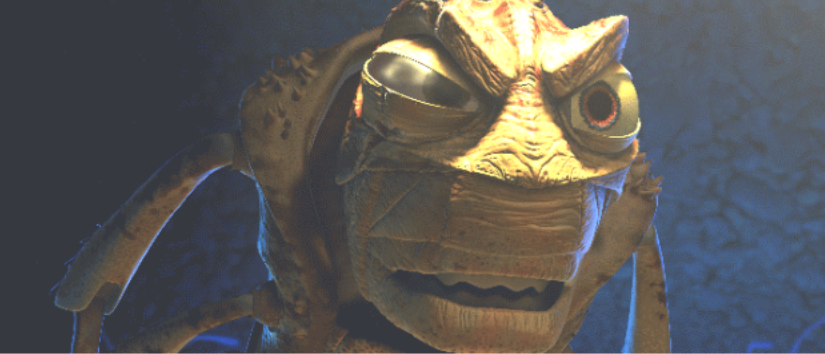
\includegraphics[width=0.7\textwidth]{Bilder/hopper.PNG}
	\caption{The contrast in lighting emphasizes Hopper from "A Bug's Life" \cite{bugslife}}
	\label{fig:hopper}
\end{figure}

Note the strong key light, which illuminates the character from above and leaves some areas of his face in shadow. In addition, the character has a strong rim light, which makes him stand out against the background. All other areas in the scene are more weakly lit. Even if the background now contains many elements, there is a strong focus on the character in focus.\\

Another visual effect to control the player's attention is playing with size differences and their weighting \cite{sudeep}. The following scene (see Figure \ref{fig:klee}) from the Pixar movie "A bugs life" will serve as an example: An ant standing on a cloverleaf is shown. The perspective in which the camera is placed and the shadow of the ant gives the viewer the feeling of being very small. 

\begin{figure}[H]
	\centering
		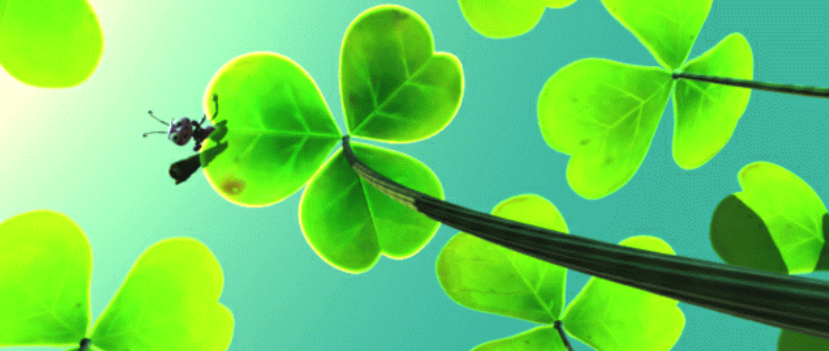
\includegraphics[width=0.7\textwidth]{Bilder/klee.PNG}
	\caption{Scale and its balance help convey a bug’s view of the world. \cite{bugslife}}
	\label{fig:klee}
\end{figure}

This helps the viewer to adjust to his surroundings and creates a unique atmosphere of being very tiny \cite{sudeep}. Also, the rim light is used here to clearly set the cloverleaf apart from the sky, which is its background. Here, the sun shines directly on the cloverleaf (illuminating it from above), which makes it stand out strongly from the rest of the scene and the sky. This brings it very much into the foreground. In this example, the sunlight is the light that makes the sides of the clover shine, thus being both key and rim light \cite{sudeep}.\\

Another goal of visual effects and especially lighting is to give a mood and atmosphere to a given scene. This can happen mainly through the use of color: Very often, for example, red lights are used to excite the viewer and leave him with an uneasy feeling \cite{Shadowplay}. Calm, peaceful, scenes, on the other hand, are often lit with high key style. The scene is flooded with soft lights, there are few shadows that could hide details of characters and colors are used that are associated with peace and tranquility \cite{sudeep} (See Figure \ref{fig:flickvshopper} and \ref{fig:friedlich}).

\begin{figure}[H]
	\centering
		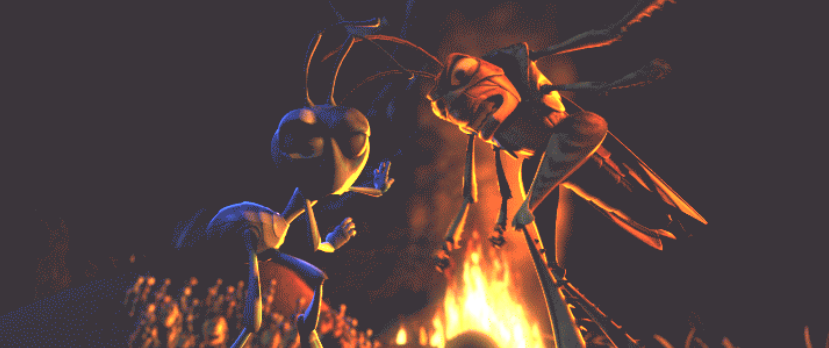
\includegraphics[width=0.7\textwidth]{Bilder/flickvshopper.PNG}
	\caption{A fight scene which is lit in low key \cite{bugslife}}
	\label{fig:flickvshopper}
\end{figure}

\begin{figure}[H]
	\centering
		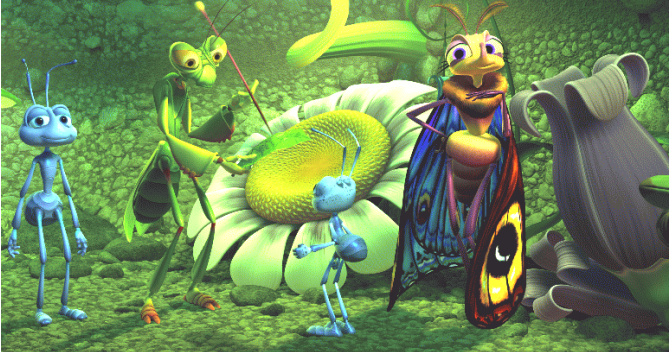
\includegraphics[width=0.7\textwidth]{Bilder/friedlich.PNG}
	\caption{A peaceful scene which is illuminated using high key techniques \cite{bugslife}}
	\label{fig:friedlich}
\end{figure}

Finally, another technique can be used to create a desired atmosphere: The use of shadows. Hard and distant light sources create crisp shadows. These produce a cold, sterile scene, giving the viewer or player an uncomfortable feeling. The shadows in Figure \ref{fig:sleeping} help evoke a dark, lonely atmosphere. Here, the glow of the television is the primary source of light, and the sleeping character casts an striking shadow on his couch. This arrangement of shadows, white lights and also the choosen perceptive arouses a lonely mood \cite{sudeep}. 
Notice how in this scene the character misses an rim light. This lets the character visually sink into his couch. 
\begin{figure}[H]
	\centering
		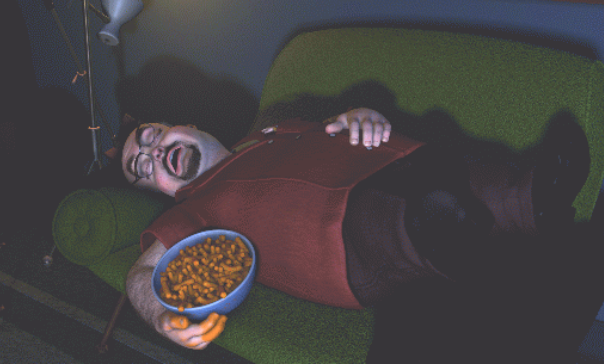
\includegraphics[width=0.7\textwidth]{Bilder/sleeping.PNG}
	\caption{Light from the TV casting shadows on a sleeping character from "Toy Story" \cite{toystory}}
	\label{fig:sleeping}
\end{figure}



On the other end of the spectrum, soft lights are used in warm and pleasing scenes because they create faint, barely noticeable  shadows \cite{Shadowplay} \cite{sudeep}.
    \chapter{Application in a serious Game}
In the course of the last chapters of this seminar work, many techniques to convey a desired atmosphere have been talked about and presented. Therefore, some applications of these techniques will now be illustrated by a real example. A serious game, which was also developed in the context of this seminar paper, will serve as an illustrative object. \\

The underlying game represents a serious game. Serious games are computer games whose main objective is not the pure entertainment of the player, but rather a therapeutic, educational or didactic value \cite{serious}. The serious game shown here aims to be used in the therapy of the hoarding disorder. \\\\
In short, the game is used to confront a patient with an unorganized, dirty apartment. He is then asked to tidy it up bit by bit. Initially, the atmosphere of the game scene, i.e. his virtual apartment, is supposed to appear very grim and dystopian. In the course of the game, the more the player brings order to the scene, the more pleasant and lighter the atmosphere should become. This effect is mainly created by some applications through above mentioned scene lighting techniques. The game itself was developed by a student team at Kempten University of Applied Sciences in cooperation with the "vfkv - Ausbildungsinstitut München gGmbH". The goal was to use the game to accompany during therapy under the supervision of a therapist.
\begin{figure}[H]
	\centering
		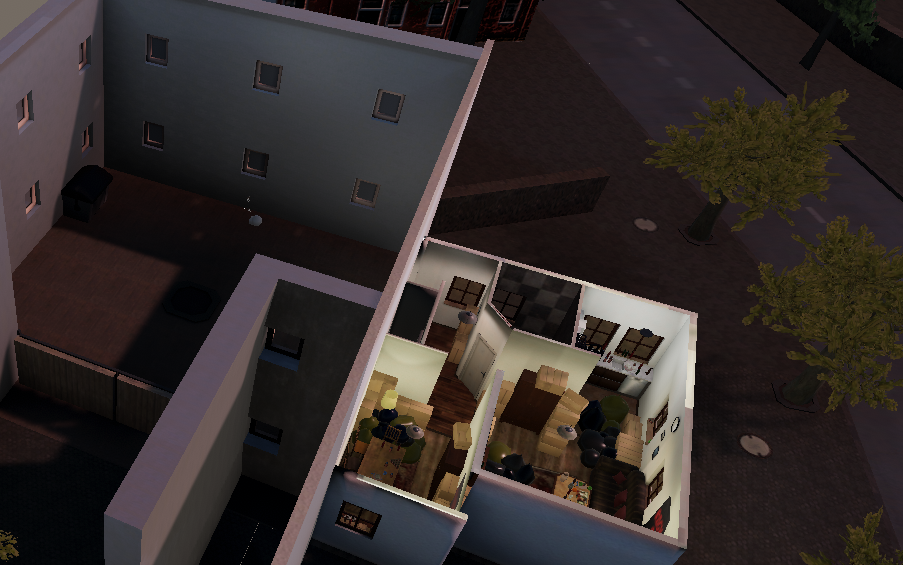
\includegraphics[width=0.7\textwidth]{Bilder/Erfassen.PNG}
	\caption{The game is divided into two scenes. The apartment and a courtyard. }
	\label{fig:szenes}
\end{figure}
\newpage
At first, the player stands in a courtyard to his virtual apartment. He sees a door, which is illuminated with a light directly above it. Although the light is not extremely strong, it already represents a key light, which draws attention to this door. This establishes it as a point of interest for the player. Since it is used to start the therapy, this effect is also very intentional. \\

\begin{figure}[H]
	\centering
		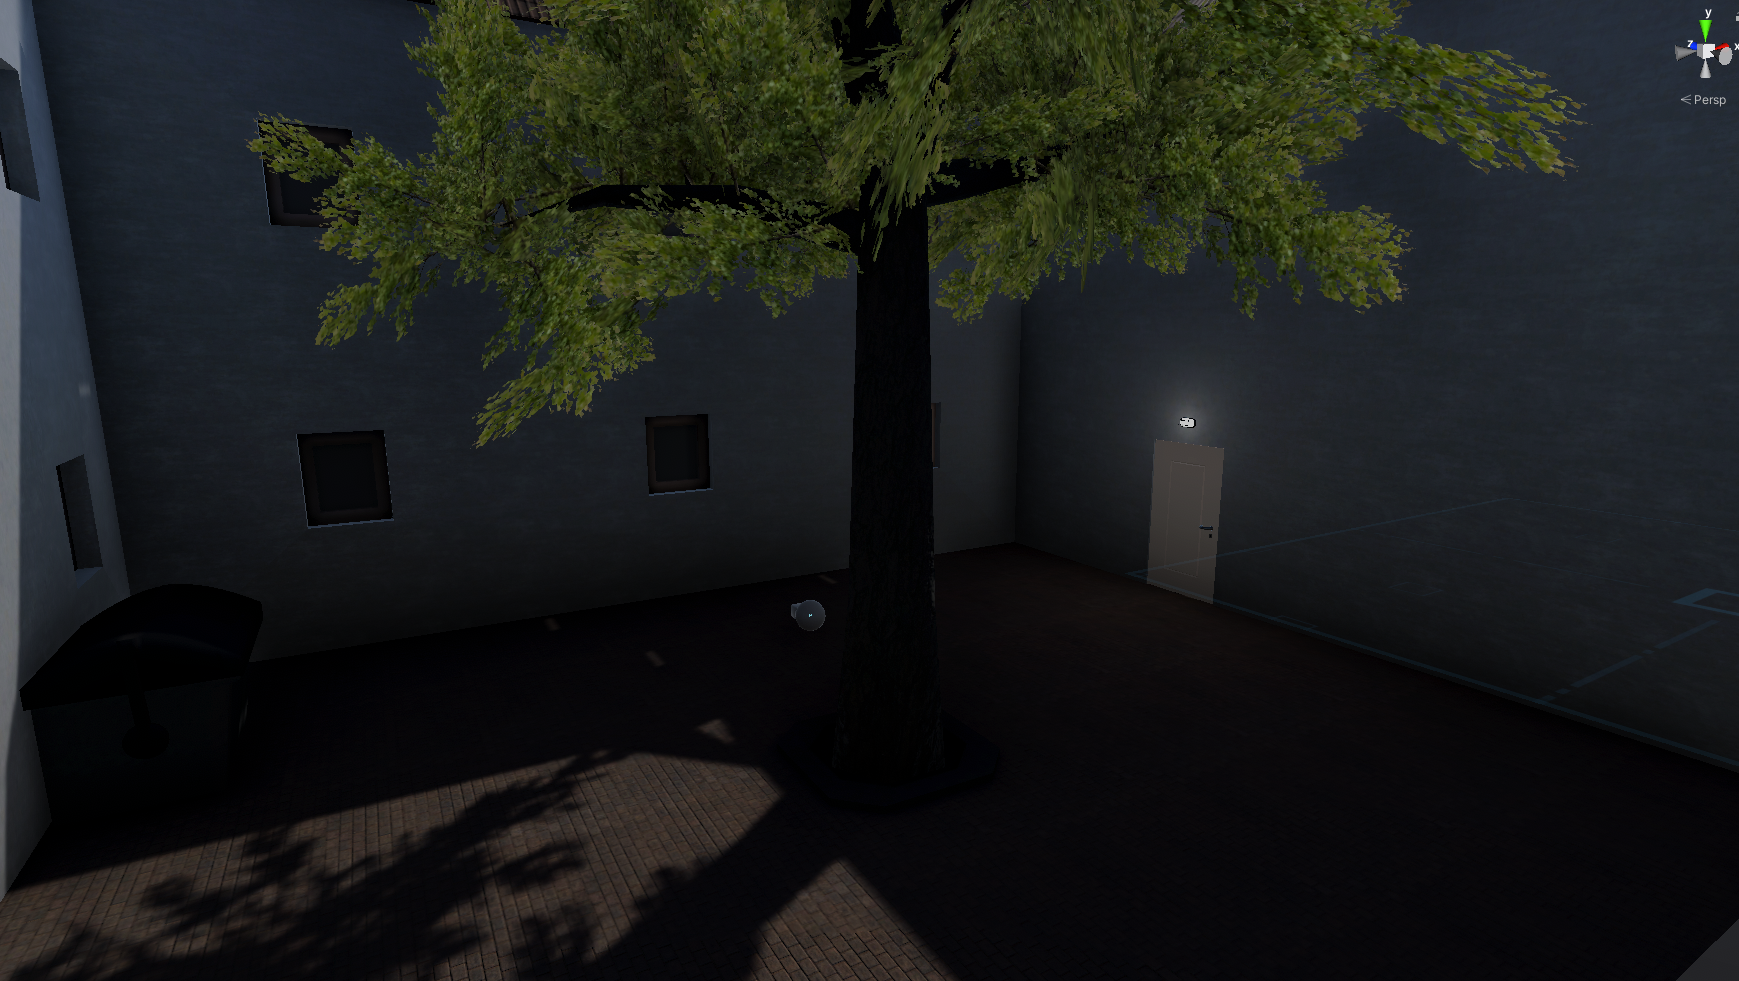
\includegraphics[width=0.7\textwidth]{Bilder/Innenhof keylight.PNG}
	\caption{The courtyard and a the door with a keylight above it. }
	\label{fig:door}
\end{figure}


The therapist, which can influence the gameplay at all times, has the possibility to give the player visual hints on how to navigate the level. These visual hints are described further in section \ref{chap:witcher} of this paper. \\
In addition, the therapist can add a yellow rim to objects that the player should interact with. This not only guides the player to this object, but also represents a rim light and hits implications made in the previous chapters (see chapter \ref{chapter:ThreePoint}). The yellow border makes the object stand out very strongly from its surroundings and can be seen very easily by the player. In addition, yellow is easily perceived as a signal color.\\
\newpage
When the player enters his virtual apartment, he is confronted ( depending on the amount of rubbish in his apartment, which is initially very large) with very dark lighting. The techniques that lead to this gloomy lighting are mainly based on the spectrum of low-key lighting.

\begin{figure}[H]
	\centering
		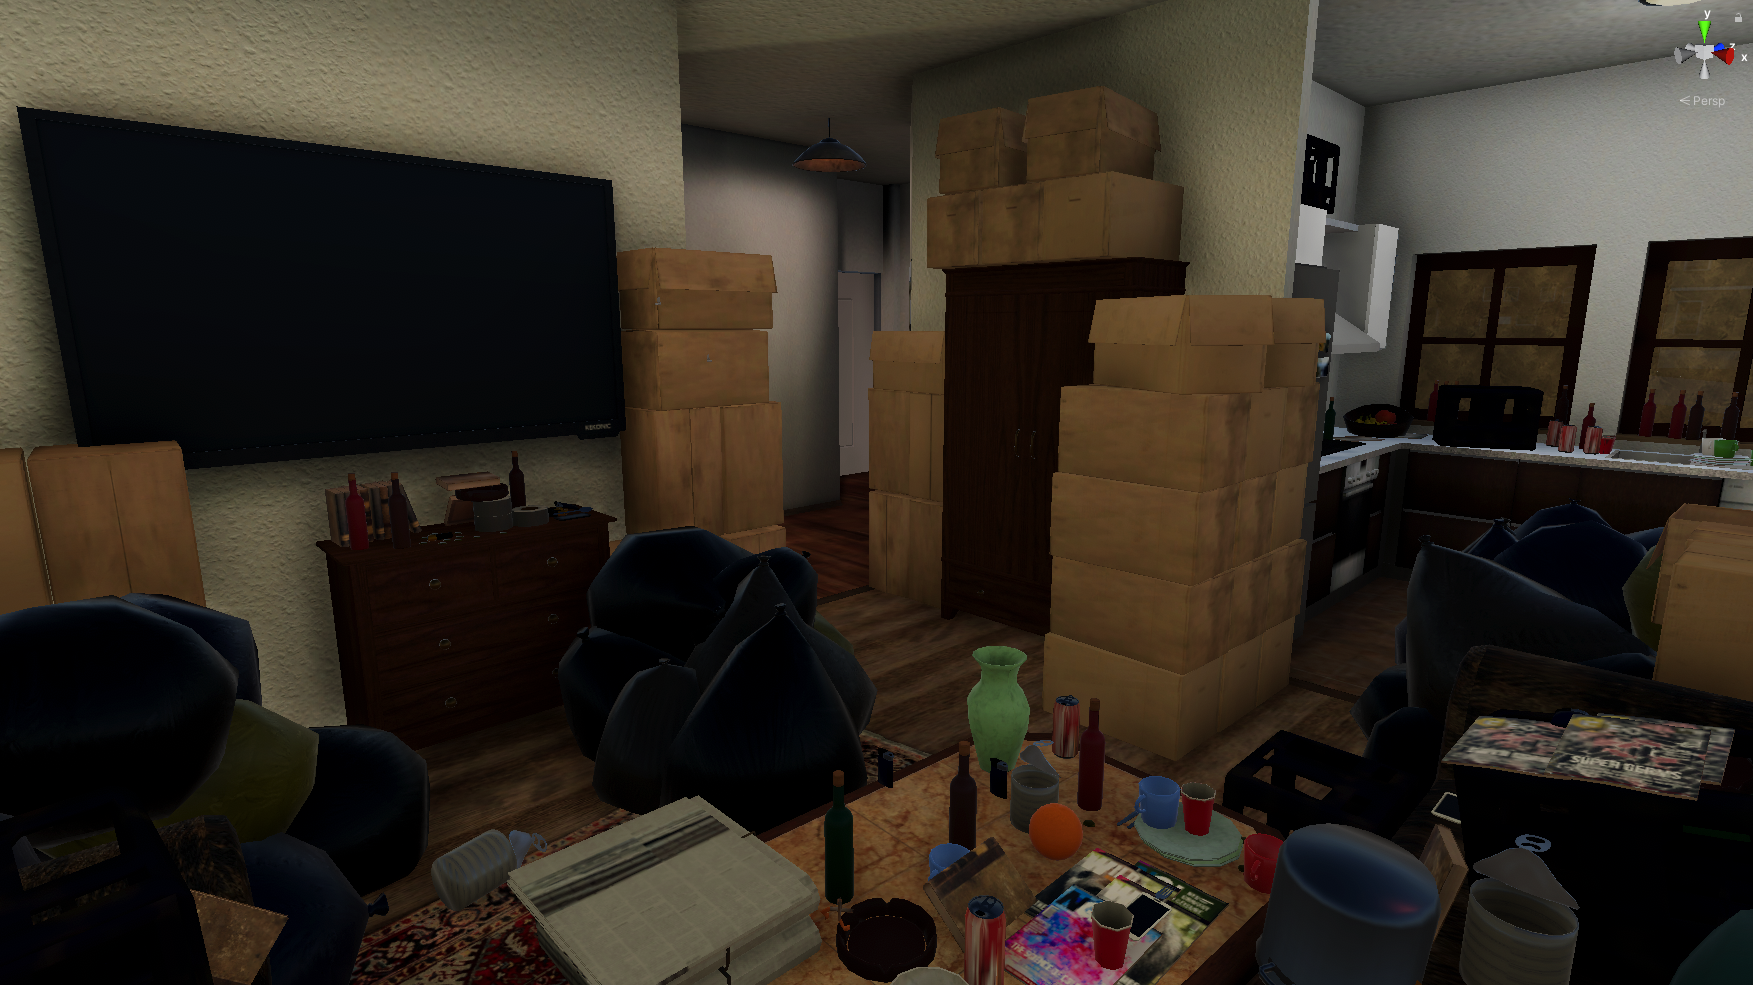
\includegraphics[width=0.7\textwidth]{Bilder/wohnzimmer Dunkel.PNG}
	\caption{An apartment which is illuminated in low key style. }
	\label{fig:darkroom}
\end{figure}
This effect is achieved by combining several techniques. Some of these will be discussed in more detail below. First, of course, the intensity of the lighting sources in the scene is adjusted. The sun in particular is a key light for the entire scene and has a very strong influence on the appearance of the apartment, which is why it is adjusted as a lighting source first of all. In addition to its intensity, the temperature of the color is also adjusted, and changed from a rather reddish tone to a bright, white and pleasant hue, making the scene generally look much brighter and much more details are visible. This represents the beginning of a transition to a high-key lighting style. 
\begin{figure}[H]
	\centering
		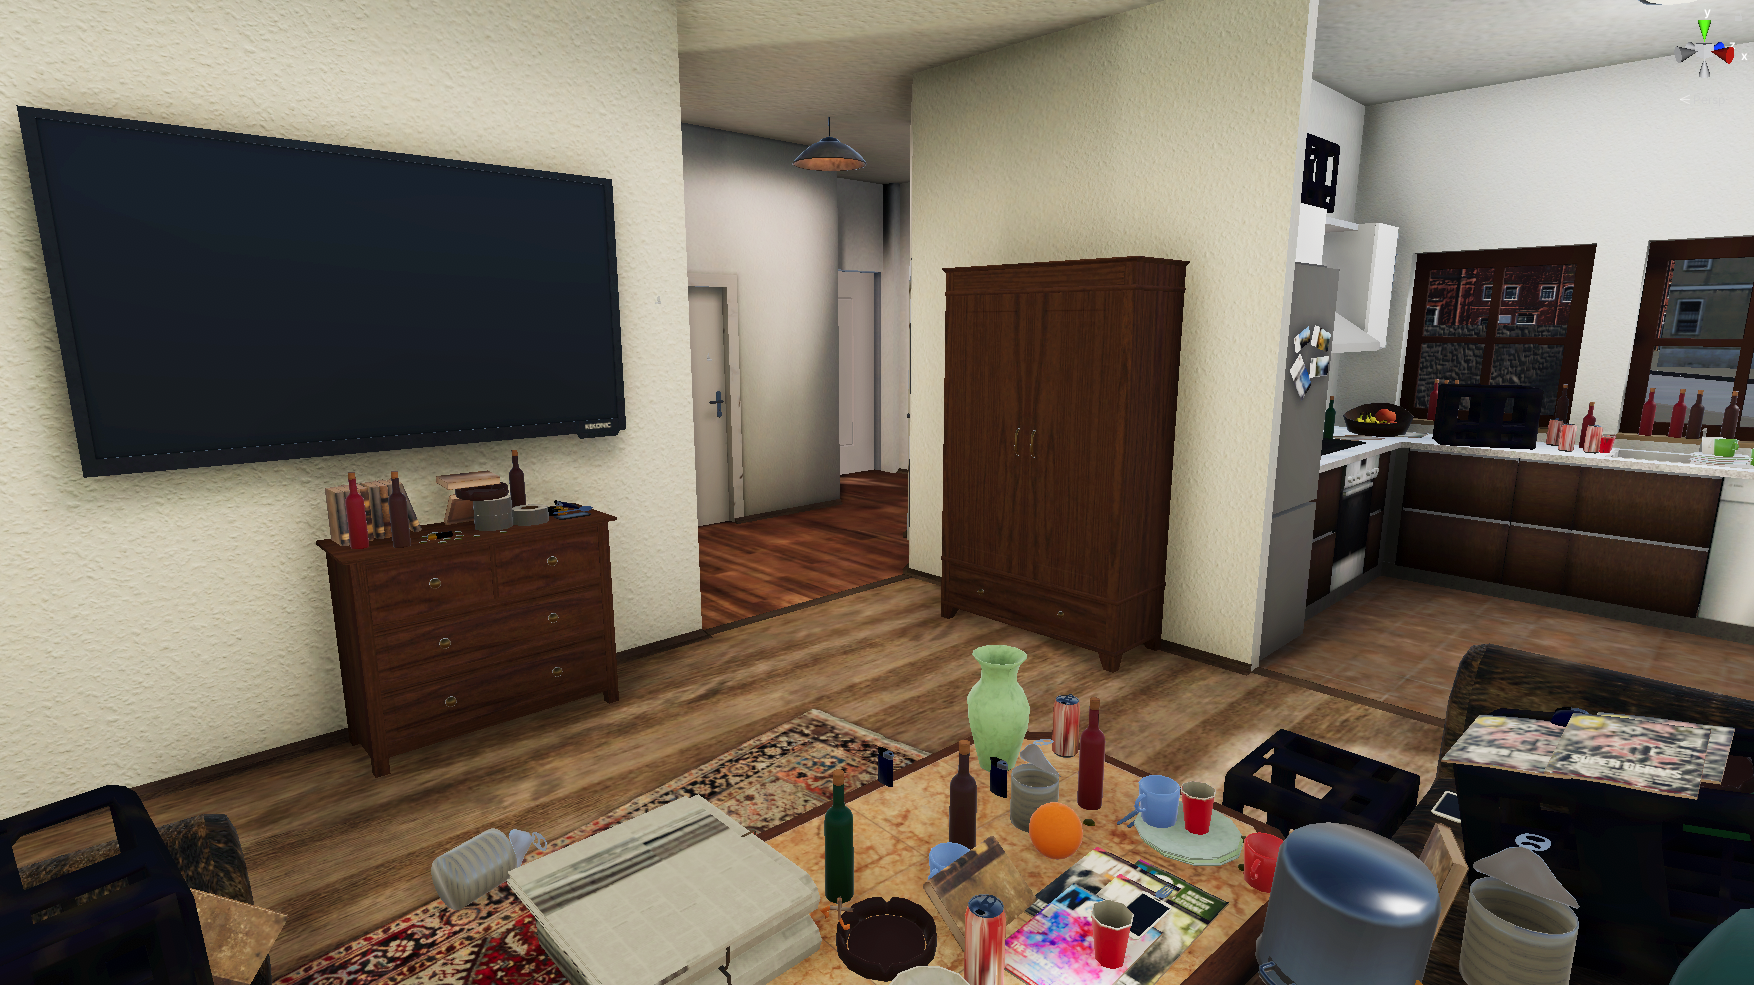
\includegraphics[width=0.7\textwidth]{Bilder/Wohnzimmer hell.PNG}
	\caption{The same apartment which is now illuminated in high key style. }
	\label{fig:darkroom}
\end{figure}
\newpage
In addition to the sun, the illuminance of the individual light sources in the apartment, i.e. ceiling lamps and floor lamps, is also adjusted and set much brighter. All of this contributes to making the scene much more enjoyable for the player. This gives him positive reinforcement, which should make him feel good every time he decides to throw an object in the trash. In addition, post-processing effects are also used. These effects ensure that the ambient light (previously also called fill light) is increased, making details of the scene much more recognizable. This can also be used as a further lever to confront the player with an increasingly better atmosphere.\\
The reason why all these efforts are made regarding the change of the light designg is, as briefly mentioned above, very simple: The more objects the player disposes of, the better and more pleasant the atmosphere of the virtual scene should become. The main reason for this is that it serves as a positive reinforcement for the patient (i.e. the player) and thus has a psychological benefit for the therapy of a messie-patient.\\
In general, an additional attempt is made to apply these effects and techniques slowly over a certain period of time. This not only leads to the generation of a visually more appealing image, but also to the fact that, in the best case, the patient only notices the change in the environment subconsciously and thus the desired illusion is maintained.
\\
    \chapter{Conclusion and Discusion}
The aim of this work was to show how a desired atmosphere can be achieved through the use of visual effects. The topic came into being because it was clear that every game creates a certain atmosphere. However, it was not clear how exactly this atmosphere can be created and which techniques have been developed for this purpose. Likewise, the goal of this work was to create a scientific vocabulary as a basis for describing such techniques. 

Therefore, the first step was to describe how lighting works in the real life and how measured values can be derived to describe just that. Then, the process of how these qualities of lighting can be simulated in the virtual world was described. With this knowledge, some techniques were then discussed by which an atmosphere can be achieved in video games, but also in the film industry, especially in animated films. \\
We have seen that by using three-point-lighting dramaturgic effects can be created, and thus the atmosphere of a scene or a game can be strongly impacted. We also looked at some ways to describe and summarize the combination of these techniques. After that, we saw how they have been applied in examples such as animated films. Finally, many of these techniques were applied in the context of a serious game, which was developed in parallel to this seminar work. \\
In the course of the work, it became especially clear that a precise scientific definition and regulation for aspects of game design and especially the creation of a desired atmosphere are missing. Even the concept of atmosphere in games is very difficult to narrow down and there are many attempts at definitions, which have also found their way into the elaboration of this work. \\
The same can be observed in the documentation of techniques used to design video games. While there are video games on the market that deliberately create a desired atmosphere and know exactly how to do it, unfortunately, these approaches are very rarely recorded in the form of scientific papers. Therefore, it was inevitable to make use of the work of film and even photography. However, as seen in the last chapter, it is partly very easy and intuitive to apply these techniques to video games.\\
\newpage
Finally, as the author, I would like to have my seminar paper briefly revisited again and express some thoughts. At the beginning it was very difficult to find a starting point for the research. There were some websites and especially YouTube videos that dealt with this topic, but I could not draw any empirical benefit from them, which is why they served as inspiration for some approaches, but by no means as a source. Therefore, and for the reason that these very effects were used in the accompanying development of a serious game, I decided to dive into the basics of lighting and describe them in great detail. Thus, the goal and title of this work was to show basic visual effects for creating a desired atmosphere and to explain their use. In my opinion, this goal was achieved. \\\\

As a final outlook, it remains to mention that one can be very excited about the further development of the artistic aspects of a video game. Especially when these are finally put down on paper.
    %\input{./Bestandteile/main}
% ----------------------------------------------
    \listoffigures  					 	        % Abbildungsverzeichnis
    \clearpage
    %\listoftables						            % Tabellenverzeichnis 
    \clearpage
\backmatter 

% Bitte Zitierstil mit Betreuer absprechen! Möglich sind z.B.
%\bibliographystyle{natdin}
%\bibliographystyle{abbrvdin}			
%\bibliographystyle{alphadin}		% Zitierstil des Literaturverzeichnisses

\bibliography{./Literatur/quellen}	% Literatur (BibTex) einbinden 
\bibliographystyle{ieeetr}
\newpage
\thispagestyle{empty}

% Bitte hier keine Änderungen vornehmen, sondern vollständig handschriftlich ausfüllen

\noindent  {\Large \textbf{Erklärung}}\\ 

\vspace*{2cm}

\noindent
Hiermit versichere ich, dass ich die vorliegende Arbeit selbstständig angefertigt, 
nicht anderweitig für Prüfungszwecke vorgelegt, alle benutzten
Quellen und Hilfsmittel angegeben, sowie wörtliche und sinngemäße Zitate gekennzeichnet habe.
\vspace{2cm}

\noindent
Kempten, den 09. Juli 2021
\hspace*{2cm}%
\dotfill\\
\hspace*{8.5cm}%
\textit{Unterschrift des Verfassers}

\vspace*{5cm}

\noindent  {\Large \textbf{Ermächtigung}}\\ 

\vspace*{2cm}

\noindent
Hiermit ermächtige ich die Hochschule Kempten zur Veröffentlichung der Kurzzusammen-
fassung (Abstract) meiner Arbeit, z. Bsp. auf gedruckten Medien oder auf einer Internet-
seite.
\vspace{2cm}

\noindent
Kempten, den 09. Juli 2021
\hspace*{2cm}%
\dotfill\\
\hspace*{8.5cm}%
\textit{Unterschrift des Verfassers}
 	% Erklärungen - Unterschreiben nicht vergessen!

\end{document}